\section{Results}
\label{sec:evaluation-results}
The analysis of results consisted in the last phase of the study; during this phase data have been manipulated and transformed into aggregated data by the authors. We analyzed each participant's screen recording to calculate the task completion rate and report this measure, in conjunction with the duration of each task, in a spreadsheet; the same operation happens for the SUS Score, automatically computed by the remote testing platform according to Brooke's formula \cite{brooke_sus_1996}, and the demographic answers. Eventually, qualitative answers are reported and correlated with quantitative results.

\subsection*{Participants}
We carried out the study with nine participants (2 women and 7 men) between 23 and 30 years old, three of which with a computer science background but only two belong to user profile P2, i.e. with experience in the AR/VR development field. We believe that, according to Nielsen et al. \cite{nielsen_mathematical_model_usability}, nine participants are enough to cover all the usability issues, where their model showed that five to eight participants can identify 80-85\% of these problems.

\subsection{Quantitative Results}
\subsubsection*{Effectiveness}
In order to measure the effectiveness through the task completion rate, we identified shorter operations per each task (\emph{sub-tasks}) and rated each participants' task by marking which of these sub-tasks has been performed, then calculating the ratio over the total number of sub-tasks. The number of operations per task are summarized as follows, while their detailed list is included in \autoref{appendix:subtasks}: Task 1 (9 sub-tasks), Task 2 (10 sub-tasks), Task 3 (10 sub-tasks), Task 4 (11 sub-tasks).

In the measurement of the effectiveness contributed only eight over nine participants, due to a technical issue that did not allow the playback of user's screen recording and its consequently analysis of the tasks. However we decided to include this participant's metrics for the next quantitative and qualitative measurements. The final effectiveness, measured as the average of task-related effectiveness (\autoref{tab:avg-effectiveness}), is 92,93\% showing that, overall, participants performed well in the study execution as also demonstrated by \autoref{fig:task-participant-effectiveness}.
\begin{table}[H]
    \centering
    \begin{tabular}{lr}
    \hline
           & \multicolumn{1}{l}{Effectiveness (Average Task Completion Rate)} \\ \hline
    Task 1 & 95,83\% (SD = 11,79\%)                                           \\
    Task 2 & 96,25\% (SD = 10,61\%)                                           \\
    Task 3 & 88,75\% (SD = 8,35\%)                                            \\
    Task 4 & 90,91\% (SD = 10,87\%)                                           \\ \hline
    \end{tabular}
    \caption{Effectiveness per task}
    \label{tab:avg-effectiveness}
\end{table}

\begin{figure}[H]
    \centering
    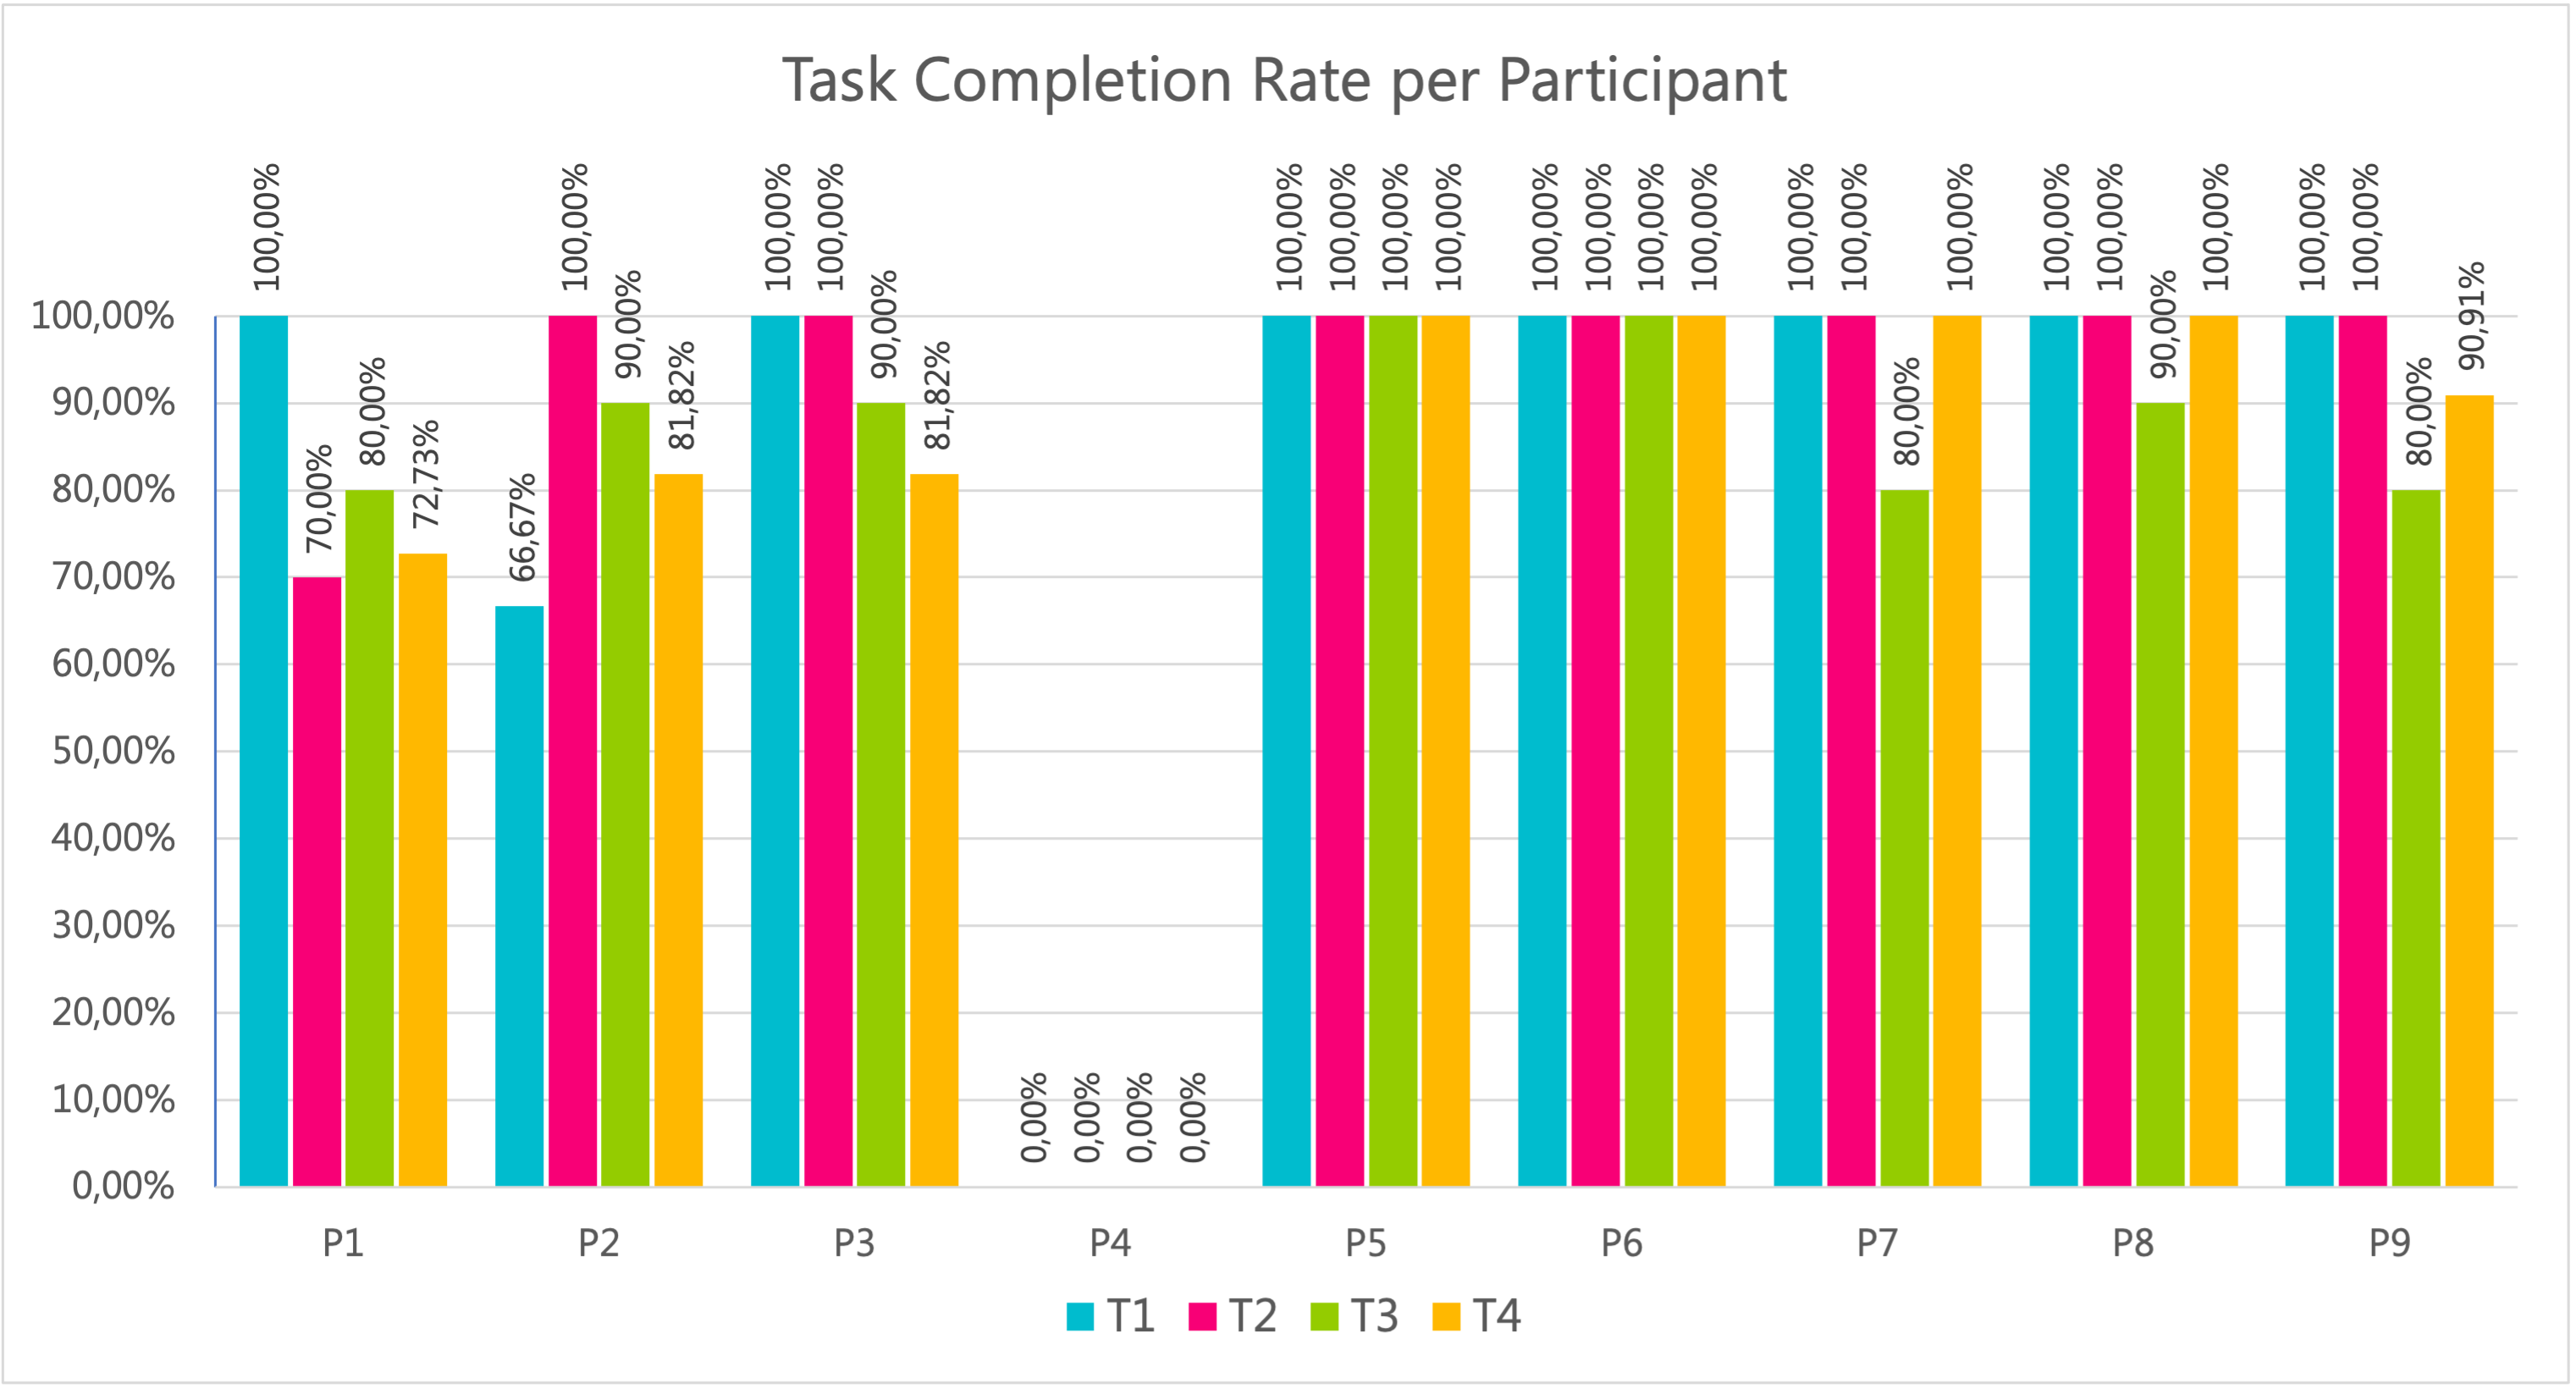
\includegraphics[width=\linewidth]{Figures/Evaluation/results/task-completion-rate_per-participant.png}
    \caption{Task Completion Rate per Participant}
    \label{fig:task-participant-effectiveness}
\end{figure}
Among the tasks, it resulted that the first two were completed with less problems than the third and fourth ones, in detail only participants 1 and 2 had problems, respectively, with task 2 and task 1 while all the other participants achieved 100\% of completed sub-tasks. The last two tasks, however, were completed with a slightly smaller effectiveness but still they proved that users were able also to manage more complex modelled experiences.

\subsubsection*{Efficiency}
\autoref{fig:completion-times} shows the average time required by users to complete each task with its standard deviation, resulting in an average efficiency of 398 seconds (6 minutes 38 seconds) per task per participant.
\begin{table}[h]
\centering
\begin{tabular}{lr}
\hline
       & \multicolumn{1}{l}{Efficiency (average task completion time)} \\ \hline
Task 1 & 306s (SD = 103,56s)                                           \\
Task 2 & 354s (SD = 109,40s)                                           \\
Task 3 & 522s (SD = 168,84s)                                           \\
Task 4 & 410s (SD = 116,13s)                                           \\ \hline
\end{tabular}
\caption{Efficiency per task}
\label{tab:avg-efficiency}
\end{table}

\begin{figure}[htbp]
    \centering
    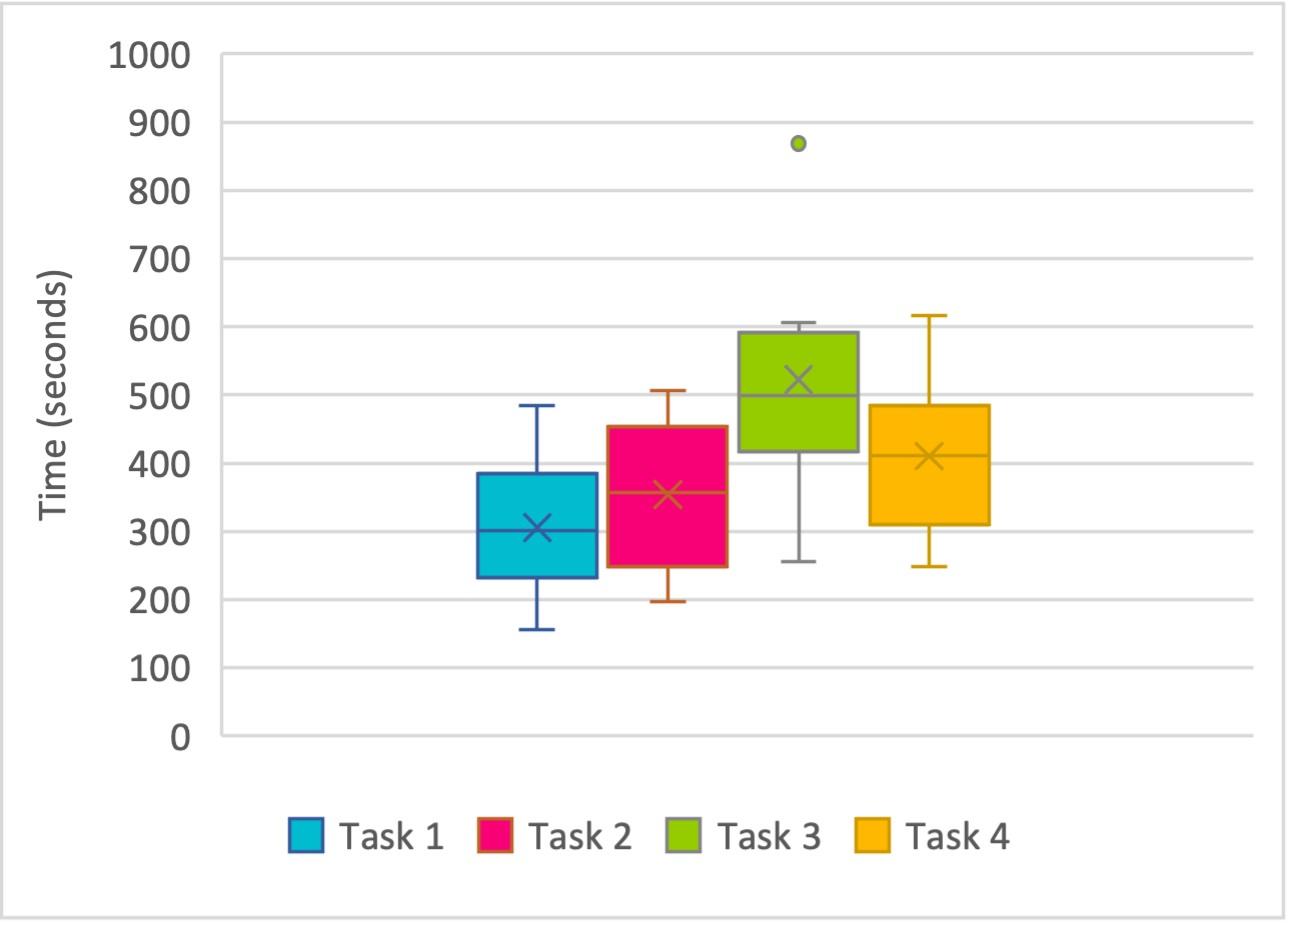
\includegraphics[width=0.8\linewidth]{Figures/Evaluation/results/completion-times.png}
    \caption{Completion times per task (in seconds)}
    \label{fig:completion-times}
\end{figure}
By comparing the average efficiency values (\autoref{tab:avg-efficiency}) with the effectiveness (\autoref{tab:avg-effectiveness}) it is possible to notice that participants six and eight achieved the highest rate of effectiveness per completion time. Even though their profile (P2) sample is too small to draw rigorous conclusions, this detail might suggest that their experience in computer science and AR/VR development results in better performances in efficiency and effectiveness than non-expert users. However, further research is needed to validate this hypothesis.
\begin{figure}[htbp]
    \centering
    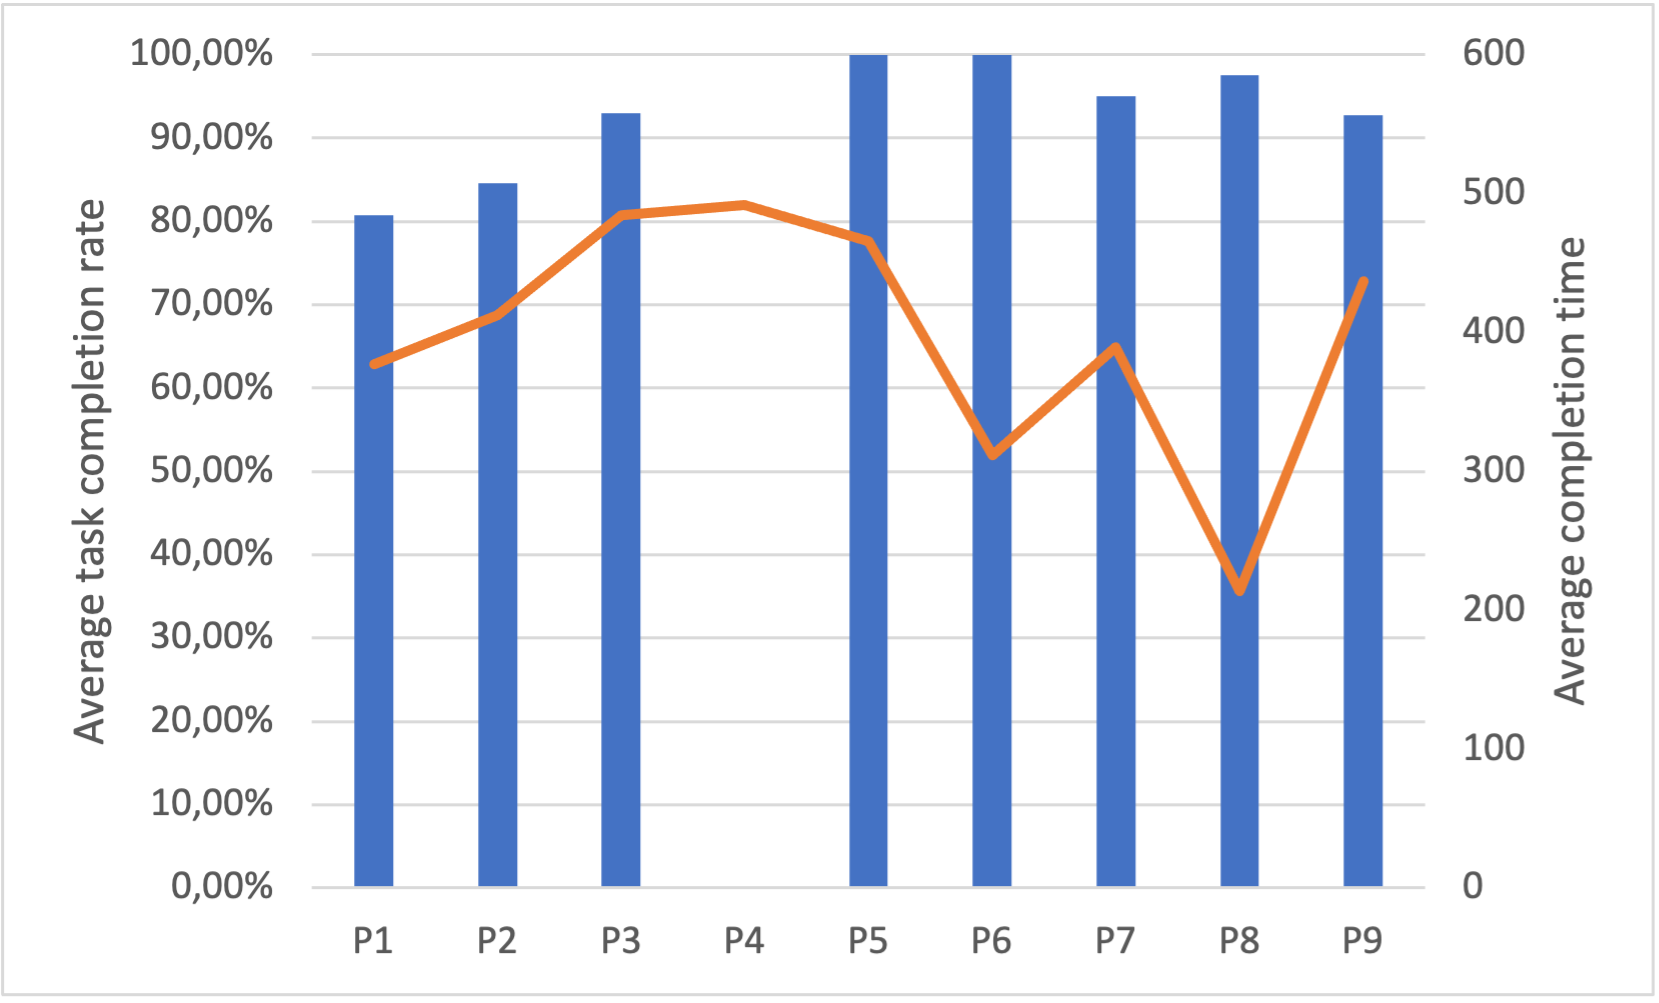
\includegraphics{Figures/Evaluation/results/completion-rate-time.png}
    \caption{Comparison of effectiveness and efficiency per participant}
    \label{fig:completion-rate-times}
\end{figure}

\subsubsection*{Satisfaction}
The \gls{SUS} Questionnaire obtained an average score of 75.0/100.0 with a standard deviation of 11.2\%, a minimum rating of 62.5/100.0 and a highest score of 100.0/100.0 (\autoref{fig:sus-results}).
\begin{figure}[h]
    \centering
    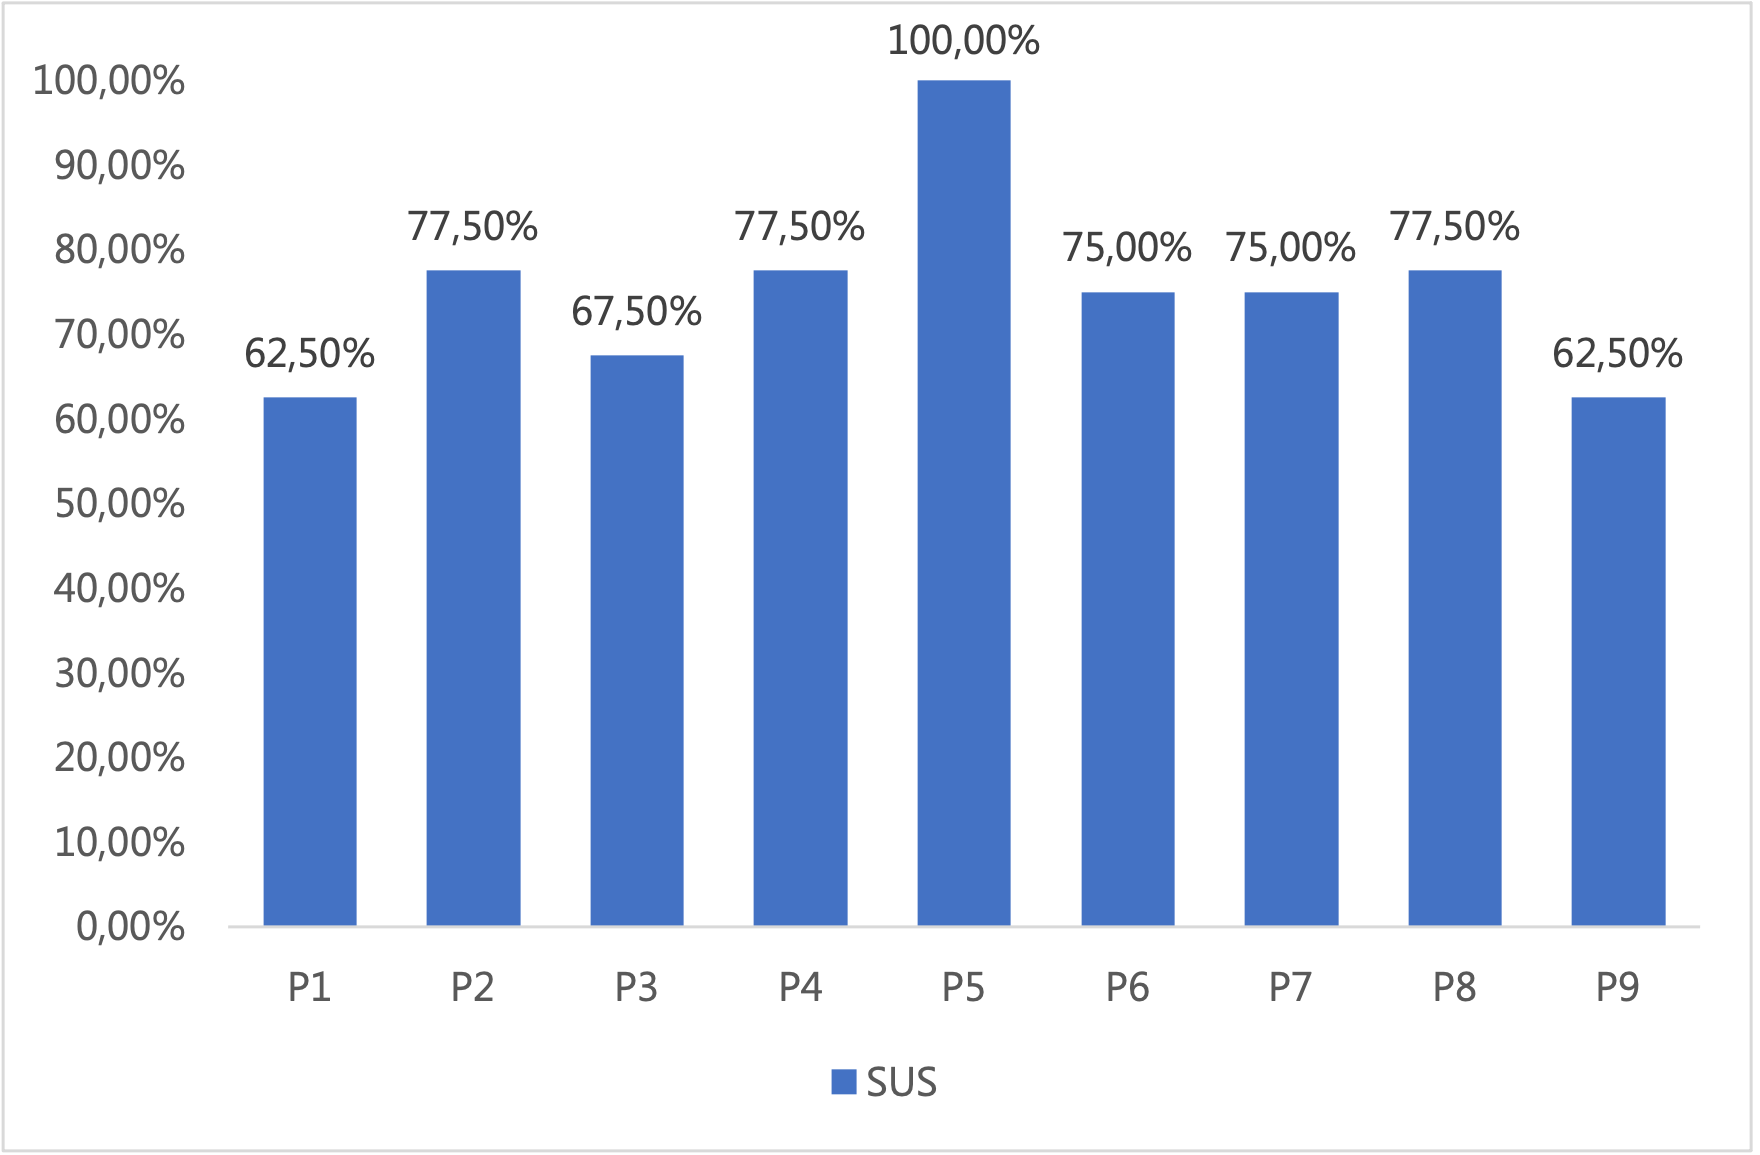
\includegraphics{Figures/Evaluation/results/sus.png}
    \caption{SUS Score Distribution}
    \label{fig:sus-results}
\end{figure}

The \glsxtrlong{SUS} is an effective and low-cost tool to assess the usability of a product, yet it is not intuitive how to relate the numeric 100-points scale to an absolute judgement. That being the case, basing our evaluation on the work of Bangor et al.~\cite{bangor_determining_2009} we adopted their adjective rating and acceptability scale models in \autoref{fig:bangor-sus} to provide a qualitative judgement based on quantitative results. The overall outcome of the questionnaire can then be evaluated as a "Highly Acceptable" and "Good" editor's usability as perceived from users.

\begin{figure}[h]
    \centering
    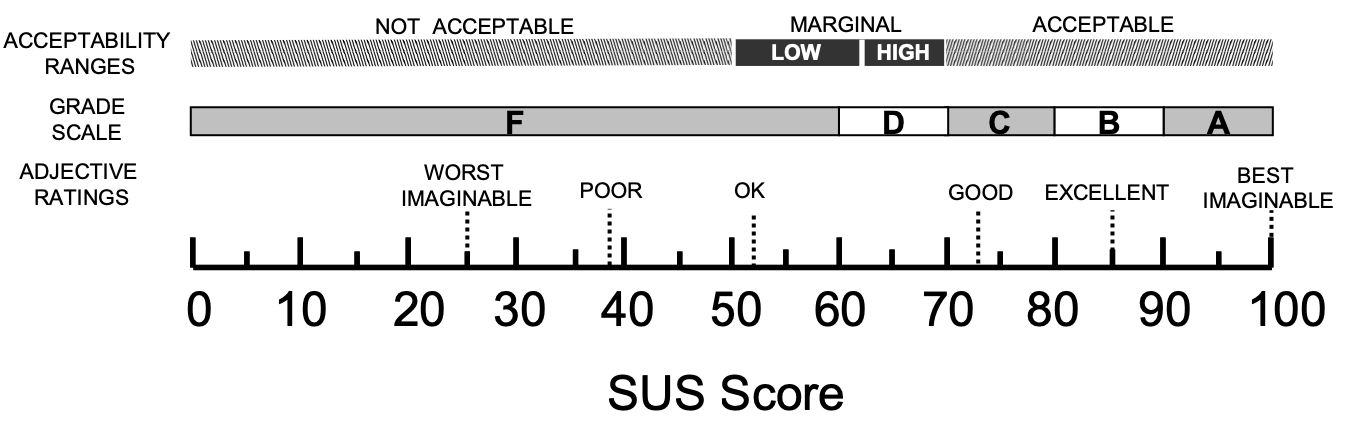
\includegraphics[width=\linewidth]{Figures/Evaluation/results/bangor-sus.png}
    \caption{A comparison of acceptability ranges, grade scale and adjective ratings with SUS Score \cite{bangor_determining_2009}}
    \label{fig:bangor-sus}
\end{figure}

\subsection{Qualitative Results}
From the qualitative open ended questionnaire we collected some users' feedback regarding the experience in using the tool. Starting from the answers regarding general problems during the use of the tool, no users found difficulties in completing the tasks but some, instead, had difficulties in dragging and dropping elements into the diagram due to the number of warning messages appearing on the top right corner of the application. These messages occur when logical rules regarding connections among elements and tags are validated, i.e. during the drag movement, resulting in potential multiple warnings. 

Other critiques regarded the few information given by the video tutorial or the ambiguity of some task descriptions; at the same time, other comments instead dissent from these opinions underlining the lack of problems faced and the conciseness of the tutorial.

The analysis of the second open ended question on positive comments about the experience showed how much participants liked using the ART Editor, defining it "Not too much complicated" (Participant 1) and "Easy to use after watching the tutorial, could be used also from people not used to this kind of tool" (Participant 2). 

Overall, then, we consider these answers as a validation of the quantitative usability test results, especially the ones on effectiveness and satisfaction, that confirmed how high scores have been achieved thanks to "The simplicity of use and the fact that there are all the things you need to build a scene in XR" (Participant 6).

Coming to the further general feedback and comments question, few users gave suggestions on possible improvements: one user pointed that sometimes, after a mistake, it is difficult to understand how to delete the last action performed (there are no 'undo' and 'redo' buttons) while another user found the application's \gls{GUI} acceptable for a prototype but less attractive if implemented for a future commercial product. 

The last constructing comment was on the role of 3D Scenes as containers of virtual elements, and the lack of clarity on what happens when elements belongs to each scene -- more specifically, it is not clear what happens if a scene is hidden but the elements in it are not. To answer this, we believe a better explanation in the tutorial on scenes and their properties should be given, in order to let other users understand that hidden scenes override the visibility property of their components.

\subsection{Findings and Next Improvements}
From the answers of the qualitative study we highlighted some improvements that could be done to the platform in order to enrich its correctness and usability: firstly the logical rules validation should happen only when elements are dropped to avoid disturbing and incoherent warning messages during user interactions; a second useful feature would be the presence of a logging tool that allows to undo and redo adjustments to the diagram. In conclusion a third feature could be a better representation of 3D Scenes as nodes more than elements as the others composing a scene; in this way it is easier to understand the concept of scenes and place the elements inside them.
Other findings have been reported while analyzing participants' screen recordings in the assessment of their effectiveness scores.

During the first task, we noted that two users didn't understand a clear distinction between state and actions, returning back several times to the task description and the tutorial to check for their definition. Only one, instead, tried to change the identifier to all the three elements regardless of their element type, resulting in the warning message "You can't set equal IDs to different object types" when trying to change the 2D Text identifier to the same of the other two 3D Models.

In the second task we noticed how, sometimes, the distinction between input and output ports in Action Nodes is not clear and should, therefore, be explained better. The last tasks showed two conceptual errors: in both the exercises two users failed in describing correctly an action first by placing two elements inside one node, resulting in their conjunction of action events rather than their disjunction, and then by modelling the opposite, i.e. a disjunction to describe a conjunction, whose effects have undefined behaviour and would be delegated on the XR Application Run-Time Engine implementation.

Finally, the sub-task output link of an Action Node to a previous State Node -- creating a loop -- has not been correctly achieved by all the participants who found other ways to represent it though, e.g. by adding a new state as the first one and linking it to the first action re-creating the loop but adding a level of redundancy. In these cases a clearer notation for parallel or exclusive actions as in BPMN could be supported, while a final diagram validation feature could minimize the number of states and actions of the \gls{FSM} and remove the redundancy issue.